\documentclass[12pt]{scrartcl}
\usepackage[sexy]{james}
\usepackage[noend]{algpseudocode}
\setlength{\marginparwidth}{2cm}
\usepackage{answers}
\usepackage{array}
\usepackage{tikz}
\usepackage{graphicx}
\newenvironment{allintypewriter}{\ttfamily}{\par}
\usepackage{listings}
\usepackage{xcolor}
\usetikzlibrary{arrows.meta}
\usepackage{color}
\usepackage{mathtools}
\newcommand{\U}{\mathcal{U}}
\newcommand{\E}{\mathbb{E}}
\usetikzlibrary{arrows}
\Newassociation{hint}{hintitem}{all-hints}
\renewcommand{\solutionextension}{out}
\renewenvironment{hintitem}[1]{\item[\bfseries #1.]}{}
\renewcommand{\O}{\mathcal{O}}
\declaretheorem[style=thmbluebox,name={Chinese Remainder Theorem}]{CRT}
\renewcommand{\theCRT}{\Alph{CRT}}
\setlength\parindent{0pt}
\usepackage{sansmath}
\usepackage{pgfplots}

\usetikzlibrary{automata}
\usetikzlibrary{positioning}  %                 ...positioning nodes
\usetikzlibrary{arrows}       %                 ...customizing arrows
\newcommand{\eqdef}{=\vcentcolon}
\newcommand{\lint}{\int_{\overset{a}{\_}}^b}
\newcommand{\uint}{\int_a^{\bar{b}}}
\newcommand{\tr}{{\rm tr\ }}
\newcommand{\im}{{\rm Im\ }}
\newcommand{\spann}{{\rm span\ }}
\newcommand{\Col}{{\rm Col\ }}
\newcommand{\Row}{{\rm Row\ }}
\newcommand{\dint}{\displaystyle\int}
\newcommand{\dt}{\ {\rm d }t}
\newcommand{\PP}{\mathbb{P}}
\newcommand{\horizontal}{\par\noindent\rule{\textwidth}{0.4pt}}
\usepackage[top=3cm,left=3cm,right=3cm,bottom=3cm]{geometry}
\newcommand{\mref}[3][red]{\hypersetup{linkcolor=#1}\cref{#2}{#3}\hypersetup{linkcolor=blue}}%<<<changed

\tikzset{node distance=4.5cm, % Minimum distance between two nodes. Change if necessary.
         every state/.style={ % Sets the properties for each state
           semithick,
           fill=cyan!40},
         initial text={},     % No label on start arrow
         double distance=4pt, % Adjust appearance of accept states
         every edge/.style={  % Sets the properties for each transition
         draw,
           ->,>=stealth',     % Makes edges directed with bold arrowheads
           auto,
           semithick}}


% Start of document.
\newcommand{\sep}{\hspace*{.5em}}

\pgfplotsset{compat=1.18}
\begin{document}
\title{MATH410: Homework 8}
\author{James Zhang\thanks{Email: \mailto{jzhang72@terpmail.umd.edu}}}
\date{\today}

\definecolor{dkgreen}{rgb}{0,0.6,0}
\definecolor{gray}{rgb}{0.5,0.5,0.5}
\definecolor{mauve}{rgb}{0.58,0,0.82}

\lstset{frame=tb,
  language=Java,
  aboveskip=3mm,
  belowskip=3mm,
  showstringspaces=false,
  columns=flexible,
  basicstyle={\small\ttfamily},
  numbers=left,
  numberstyle=\tiny\color{gray},
  keywordstyle=\color{blue},
  commentstyle=\color{dkgreen},
  stringstyle=\color{mauve},
  breaklines=true,
  breakatwhitespace=true,
  tabsize=3
}

\maketitle

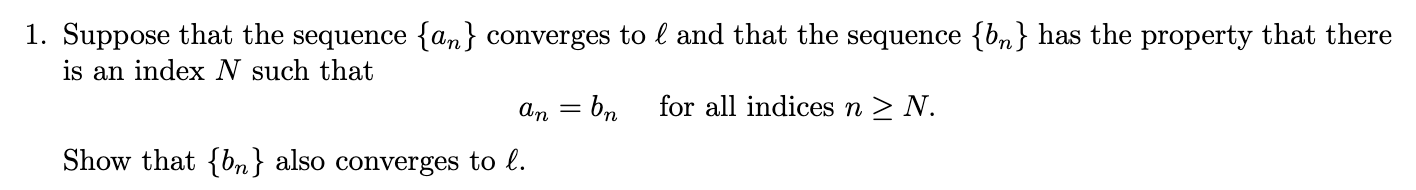
\includegraphics[width=14cm]{1.png}

\begin{proof}[Solution]

\hfill

\begin{enumerate}[a.]
  \item False. Recall in the Homework $7$ problem $5a$, we proved that $f(x) = x$
  is integrable and that $\int_a^b x dx = \frac{b^2 - a^2}{2}$. Let $a=-1, b=1$ such that 
  we want to compute $\int_{-1}^1 x dx = \frac{1^2 - (-1)^2}{2} = 0$. However, clearly, $f(x) = x \neq 0 \ \forall \ x \in (a, b)$.
  Therefore, this statement is false.
  
  \item False. Step functions are integrable but not continuous. Recall that we did a sketch of a proof in class showing that every step function is integral. 
  For the partition points inside one region, $M_i = m_i$. For the subintervals at the gaps/jumps, there are finitely many and they 
  can still be bounded using $M_i, m_i$. Therefore, $\underset{n\to\infty}{\lim}(U(f, P_n) - L(f, P_n)) = 0$ and so by the AR theorem, 
  step functions are integrable. Now we will show that a step function is not continuous. Consider a generic step function $f: [a,b] \to \RR$ with one "step."
  \[f(x) = \begin{cases}
    c, \ x \geq x_0\\
    d, \ x < x_0
  \end{cases}\]
  for some arbitrary $c, d, x_0 \in \RR, c \neq d, x_0 \in (a, b)$. Consider a sequence $\{u_n\} \to x_0$ from the right and a sequence 
  $\{v_n\} \to x_0$ from the left. Observe that $\{f(u_n)\} \to c$ and $\{f(v_n)\} \to d$. Therefore, we have found a pair of sequences that converge 
  to $x_0$, whose image sequences do not converge to $f(x_0)$. Therefore, step functions are integrable but not continous.
  \item True. Suppose $f: [a,b] \to \RR$ is integrable and $f(x) \geq 0 \ \forall \ x \in [a,b]$.
  By the AR Theorem, specifically the "moreover" part, recall that 
  \[\int_a^b f = \lim_{n\to\infty} U(f, P_n)\]
  for some partition $P_n$ on $[a,b]$. Note that 
  \[\lim_{n\to\infty}U(f, P_n) = \lim_{n\to\infty} \sum_{i=1}^n M_i(x_i - x_{i-1})\]
  by definition of Darboux Upper Sums. $M_i \geq 0 \ \forall \ i$ because $f(x) \geq 0 \ \forall \ x$. Further note that 
  $x_i - x_{i-1} > 0 \ \forall \ i$ by properties of partitions. Therefore, 
  \[M_i(x_i - x_{i-1}) \geq 0 \ \forall \ i\]
  Therefore, the sum and then limit of $n$ positive terms must also be positive.
  \[\int_a^b f = \lim_{n\to\infty}U(f, P_n) = \lim_{n\to\infty} \sum_{i=1}^n M_i(x_i - x_{i-1}) \geq 0 \implies \int_a^b f \geq 0\]
  
  
  \item False. Define $f: (0, 1) \to \RR$ such that $f(x) = \frac{1}{x} \ \forall \ x \in (0, 1)$. By limit properties, 
  \[\lim_{x \to 0} \frac{1}{x} = \infty\]
  and so $f$ is not bounded. Alternatively, suppose on the contary that $f$ was bounded, so $\exists M \in \RR^+$ such that 
  $|f(x)| = |\frac{1}{x}| \leq M \ \forall \ x \in (0, 1)$. Consider $x_0 = \frac{1}{M + 1} \in (0, 1)$ because $M > 0$.
  Then
  \[|f(x_0)| = |\frac{1}{\frac{1}{M + 1}}| = |M + 1| = M + 1 \leq M\]
  is a contradiction, and so $f(x) = \frac{1}{x}$ is not bounded on $(0, 1)$ and we have proved this statement false by counter example.
  
  \item True. Since $f$ is continuous on $[a,b]$, $f$ must attain all values from $f(a)$ to $f(b)$ and note that these image 
  values are themselves an interval, $f([a, b])$. Note that this interval is closed, and recall that all closed intervals attain a maximum
  and a minimum, which we will denote $M$ and $m$, respectively. Let $L = \max(|M|, |m|)$. By definition of max and min,
  \[m \leq f(x) \leq M \ \forall \ x \in [a,b]\]
  By substitution for $L$, 
  \[-L \leq f(x) \leq L \ \forall \ x \in [a,b]\]
  \[|f(x)| \leq L \ \forall \ x \in [a,b]\]
  and so $f$ is bounded.
\end{enumerate}
  
\end{proof}

\newpage

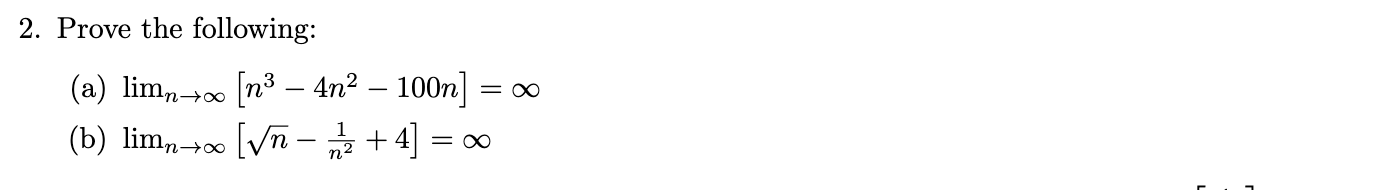
\includegraphics[width=14cm]{2.png}

\begin{proof}

\hfill

Let $P = \{0, x_1 \ldots, x_{n-1}, 1\}$ be a partition of $[0, 1]$. Since $\QQ$ and $\QQ^C$ are dense in 
each $[x_{i-1}, x_i]$, there exists a rational number and irrational number in each $[x_{i-1}, x_i]$.
Note that to show that $f: [0, 1] \to \RR$ is not integrable, we want to show that there does not exist a sequence of partitions 
$P_n$ such that $\underset{n\to\infty}{\lim}{(U(f, P_n) - L(f, P_n)) = 0}$. Observe that 
\begin{align*}
  L(f, P) = \sum_{i=1}^n m_i(x_i - x_{i-1})\\
  U(f, P) = \sum_{i=1}^n M_i(x_i - x_{i-1})
\end{align*}
where $M_i = \sup\{f(x) \ | \ x \in [x_{i-1}, x_i]\}$ and $m_i = \inf\{f(x) \ | \ x \in [x_{i-1}, x_i]\}$.
Note that $M_i = x_i \ \forall \ i$. To show this, assume on the contrary that there exists some index value 
$x_0 \in (x_{i-1}, x_i)$ such that $M_i = f(x_0) = x_0$ is the sup of the interval. Now consider the new 
interval $[x_0, x_i]$. By density of $\QQ$ once more, there exists a rational number in this interval. Denote this index 
$x_1$. Note that $x_1 > x_0 \implies f(x_1) > f(x_0)$ which contradicts that $x_0$ is the sup of the interval. Therefore, 
$x_i$ is the sup. Similarly, we can show that $m_i = -x_{i-1} \ \forall \ i$. Therefore,
\[L(f, P) = \sum_{i=1}^n -x_{i-1}(x_i - x_{i-1}) = (x_0^2 -x_0x_1) + (x_1^2 - x_1x_2) + \cdots + (x_{n-1}^2 - x_{n-1}x_n)\]
\[U(f, P) = \sum_{i=1}^n x_i(x_i - x_{i-1}) = (x_1^2 - x_0x_1) + (x_2^2 - x_1x_2) + \cdots + (x_n^2 - x_{n-1}x_n)\]
Taking their elementwise differences, observe that 
\[U(f, P) - L(f, P) = (x_1^2 - x_0^2) + (x_2^2 - x_1^2) + \cdots + (x_n^2 - x_{n-1}^2) = x_n^2 - x_0^2\]
However, $x_0 = 0$ and $x_n = 1$ by construction for our partition $P$. Therefore, 
\[U(f, P) - L(f, P) = 1^2 - 0^2 = 1 \implies \lim_{n\to\infty} (U(f, P) - L(f, P)) = 1 \neq 0\]
and so therefore, $f$ is not integrable.


\end{proof}
\newpage 

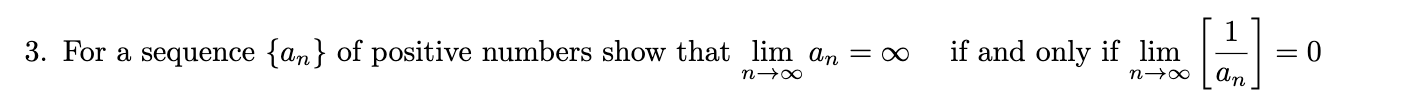
\includegraphics[width=14cm]{3.png}

\begin{proof}
  
\hfill

First, let us prove the Mean Value Theorem for Integrals (I don't think we have covered this in class). The 
MVT for Integrals states that if $f: [a,b] \to \RR$ is continuous on $(a,b)$ then there exists at least one point 
$x_0 \in (a,b)$ such that $f(x_0) = \frac{1}{b-a}\int_a^b f(x) dx$. To prove this, first apply Extreme Value theorem
such that $f$ attains a maximum and a minimum, $M$ and $m$ respectively. Therefore, 
\[m(b-a) \leq \int_a^b f \leq M(b-a)\]
Dividing both sides by $b-a$,
\[m \leq \frac{1}{b-a}\int_a^b f \leq M\]
Since $f$ is continuous, by the Intermediate Value Theorem, $f$ attains all values between $m$ and $M$, and so therefore, 
\[\exists \ x_0 \in (a,b) \text{ s.t. } f(x_0) = \frac{1}{b-a}\int_a^b f\]
and the proof is done. In the context of this problem, note that we are given that $\int_a^b f = 0$. Substituting this into the above,
\[\exists \ x_0 \in (a,b) \text{ s.t. } f(x_0) = \frac{1}{b-a}(0) \implies \exists \ x_0 \in (a,b) \text{ s.t. } f(x_0) = 0\]
as desired.


\end{proof}
\newpage

\end{document}

